\documentclass[11pt,letterpaper]{article}
\usepackage[english]{babel}
\usepackage[utf8]{inputenc}
\usepackage{fancyhdr}
\usepackage[margin=1in]{geometry}
\usepackage{enumitem}
\usepackage{amsmath}
\usepackage{graphicx}
\usepackage{setspace} 
\onehalfspacing
 
\pagestyle{fancy}
\fancyhf{}
\lhead{CS\&SS 569 HW 1}
\rhead{Nan Tang (1662478)}
\rfoot{Page \thepage}
 

\title{CS\&SS 569 Problem Set 1}
\author{Nan Tang \\ University of Washington}
\date{\today}
 
\begin{document}
\maketitle

\section*{Problem 1: Critique a VDSI}
\subsection*{Display and Explanation}

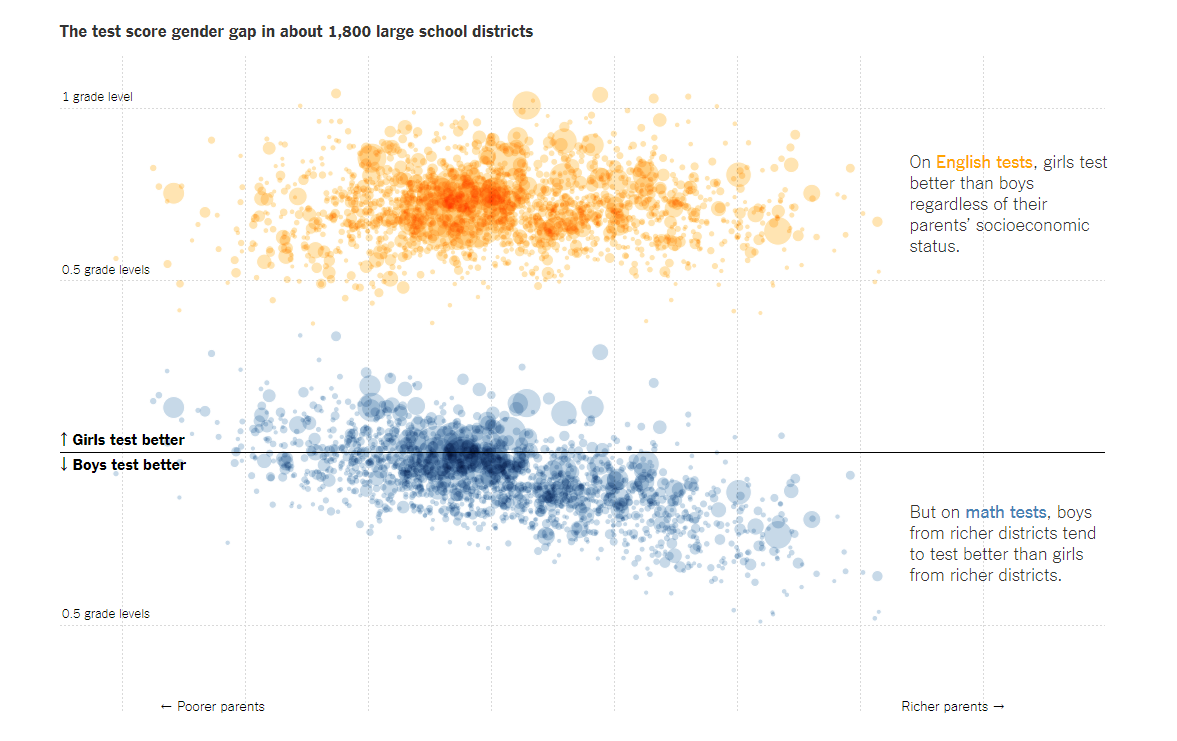
\includegraphics[scale=0.5]{display-1.png} \\

\noindent This visualization is derived from a New York Times article, \textit{Where Boys Outperform Girls in Math: Rich, White and Suburban Districts}, in June 2018. In addition to this graph, the author also provided an interactive system for viewers to search for research data of specific school districts. Combining both statistics and visuals, the article tends to convey the idea that the stereotype saying boys can do better than girls at math isn’t true for most cases of the US, however, boys who studied in rich, white and suburban districts are exceptions. The research quantified students’ ability in Math and English based on their standardized test scores for five years in one thousand school districts. They suggest that in low-income and African American districts, girls perform slightly better than boys, while boys do much better in high-income and mostly white or Asian American districts. To illustrate this point, the author compares students’ data of Montgomery Township district where median household income is high and is composed of white and Asian to districts of Detroit.

\subsection*{Interpretation and Critique}
\noindent \textbf{Scaling and Axes:} Different from ordinary cartesian plane, this graph is primarily designed to compare boy's performance in tests to that of girls in Math and English. Therefore, the scale of y-axis is considered as relative mastery of skills: x-axis represents boys perform as good as girls. If the circle is above x-axis, it represents the average performance of girls in test is better than boys, vice versa. Scaling on x-axis represents median household income in the school district. The author failed to inform the unit along x-axis, which violated the principle of scale. Possible re-scaling such as square and logarithm may cause visual distortion to viewers in this case. \\

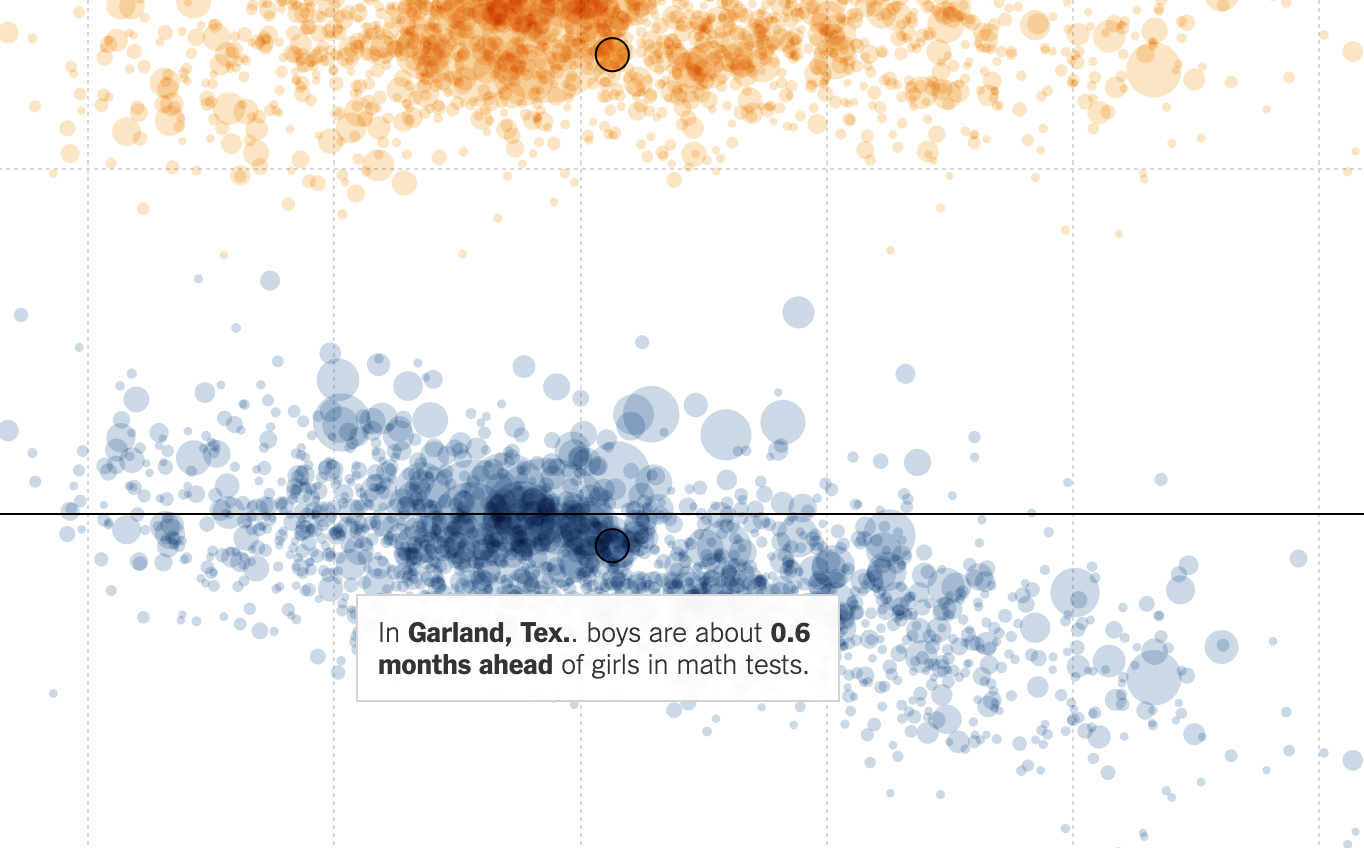
\includegraphics[scale=0.5]{display-3.png}

\noindent \textbf{Proportion of data display and chartjunk:} In the perspective of Tufte’s principles, the visualization avoids wasting area on meaningless graphics and shows richness in data display. Approximately eight percent of the area in this visualization represents the data, while interpretation concurs only a small proportion of margin. The size of each circle represents the number of students in that school district, larger the circle, more population it has. Similar to a heatmap, darker in color represents more students with akin household background and grade in tests. The interactive design enables viewers to check out details of each point, which includes the name of that school district and different genders relative performance. To sum up, this design maximizes proportion of ink on statistics display. \\

\noindent \textbf{Combination of Plots and Comparison:} In terms of expressionIn order to highlight the main conclusion of this article that boys from rich white families do better in Math than girls, the author combines students’ performance in English tests with Math. In terms of combination methods, both plots share the same scale and stretch in the same ratio, satisfying the essential requirement of scientific visuals. However, simply comparing two courses cannot come up with the conclusion that rich families focus more on boys’ education in Math. It is probable that boys from wealthy families could in average perform better than girls in multiple fields of study, which is contrary to researchers’ speculation. Hiding visuals of other subjects and taking a part for the whole, such a two-way comparison may bring distraction to viewers. \\

\noindent \textbf{Use of Number:} Instead of showing original data, average or median of test score, on the graph, the author reports the number of months ahead of boys or girls in mastery of the skill. By showing only one or two digits with at most one decimal, this step avoids potential distraction from extra digits. \\

\subsection*{Possible Improvement}
\textbf{Regression Line:} A guiding line such as linear regression or curve would make it easier for viewers to perceive relationships between those two factors. By fitting the origin data with a regression line, we can clearly convey the idea that household income and race have effects on boys' performance in Math. Meanwhile, a fitted value confidence interval is also necessary. Considering the large size of data set, it is important to visualize the uncertainty of this fitted line. \\

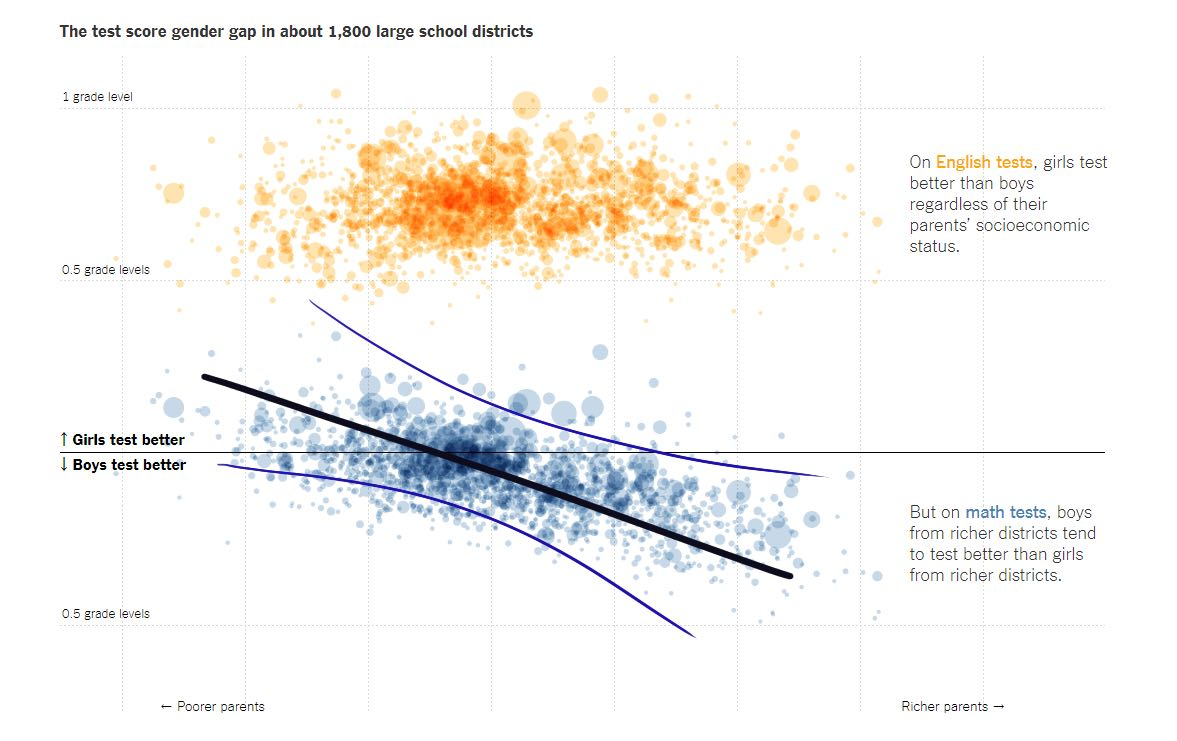
\includegraphics[scale=0.4]{improve-1.jpeg}

\noindent \textbf{Simplify Less Significant Data:} Though the topic of this article is on Math, this graph emphasizes English as well. As I mentioned in last section, the graph of English test is used as contrast. Showing as much information of the contrast as the main subject is unnecessary. I will use simple regression line instead of the complex interactive dot plot. \\

\noindent \textbf{Data Integrity:} One of the flaws of the original graph is hiding visuals of other subjects. Simply a two-way comparison will not convince the viewer of researchers' conclusion. To modify this problem, I will add regression lines of the mastery in other skills such as history, chemistry and physics to the graph, using contrasting colors. The supplement of background information will provide viewers with a holistic and objective vision on this topic of interest. 

\section*{Problem 2: Graphical Skills}
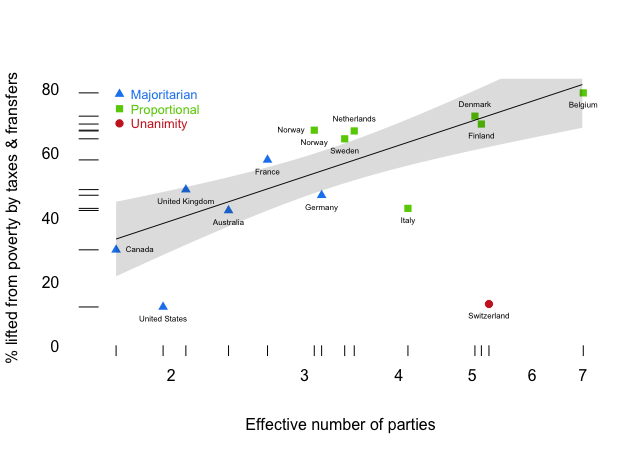
\includegraphics[scale=0.8]{problem2.png}

\begin{verbatim}
library(MASS) ## robust regression
library(Epi) ## draw shaded area

## import data 
dt1 <- read.delim("iverRevised.txt", header = TRUE, sep = ",")
dt2 <- dt1
dt2$povertyReduction <- as.numeric(dt1$povertyReduction)
dt2$effectiveParties <- as.numeric(dt1$effectiveParties)
x_dt <- dt2$effectiveParties
y_dt <- dt2$povertyReduction

## text of points
x_txt1 <- x_dt[-c(3, 4, 9, 10)]
y_txt1 <- y_dt[-c(3, 4, 9, 10)]
label_txt1 <- dt1$country[-c(3, 4, 9, 10)]

## type and color of points
pch_dt <- numeric(14)
pch_dt[dt1$partySystem=='Unanimity'] <- 19
pch_dt[dt1$partySystem=='Majoritarian'] <- 17
pch_dt[dt1$partySystem=='Proportional'] <- 15

col_dt <- numeric(14)
col_dt[dt1$partySystem=='Unanimity'] <- 'firebrick3'
col_dt[dt1$partySystem=='Majoritarian'] <- 'dodgerblue2'
col_dt[dt1$partySystem=='Proportional'] <- 'chartreuse3'

## robust regression line and confidence interval
x=x_dt[-12]
y=y_dt[-12]
lm.out <- rlm(y ~ log10(x))
newx = seq(min(x),max(x),by = 0.05)
conf_interval <- predict(lm.out, newdata=data.frame(x=newx), interval="confidence",
                         level = 0.95)

## original scatter plot
plot(x_dt, y_dt, log='x', ylim=c(0, 80), xlim=c(1.6, max(x_dt)), 
     axes=F, pch=pch_dt, col=col_dt,
     xlab='Effective number of parties',
     ylab='% lifted from poverty by taxes & fransfers')

## rescale and rename axis
axis(side=1, c(2, 3, 4, 5, 6, 7), pos=0, lty=0)
axis(side=2, c(0, 20, 40, 60, 80), las=1, lty=0)

## add annotations
text(x_txt1, y_txt1, pos=1, labels=label_txt1, cex=0.5)
text(x_dt[3], y_dt[3], pos=4, labels=dt1$country[3], cex=0.5)
text(x_dt[c(4, 9)], y_dt[c(4, 9)], pos=3, labels=dt1$country[c(4, 9)], cex=0.5)
text(x_dt[10], y_dt[10], pos=2, labels=dt1$country[10], cex=0.5)

## add fitted line and confidence interval
matshade(newx, conf_interval, col = "gray5", log='x')

## add marginal distribution
segments(x0=1, y0=y, x1=1.6, y1=y)
segments(x0=x_dt, y0=-5, x1=x_dt, y1=0)

## add legend
legend(1.65, 83, legend=c("Majoritarian", "Proportional", "Unanimity"), 
       col=c("dodgerblue2","chartreuse3","firebrick3"), 
       text.col = c("dodgerblue2","chartreuse3","firebrick3"),
       pch=c(17, 15, 19), cex=0.8, pt.cex = 1, box.lty=0)
\end{verbatim}

\end{document}